\documentclass[11pt,serif,professionalfont,aspectratio=169]{beamer}
\usepackage[T1]{fontenc}
\usepackage{concrete}
\usepackage{amsmath,amsthm,amssymb}
\usepackage{multicol}
\usepackage{caption}
\usepackage{subcaption}
%\usepackage{enumitem}
\usepackage{standalone}
\usepackage{tkz-graph}
\usepackage{tikz}
\tikzstyle{vertex}=[circle, draw, inner sep=2pt, minimum size=10pt]
\newcommand{\vertex}{\node[vertex]}
\usetikzlibrary{shapes}
\usepackage{amsfonts}
\usepackage{mathtools}
\usepackage[normalem]{ulem}
\usepackage{adjustbox, centernot}
\usepackage{wrapfig,graphicx}
\theoremstyle{plain}
  \newtheorem{conjecture}{Conjecture}
  \newtheorem{observation}{Observation}
\DeclarePairedDelimiter{\ceil}{\lceil}{\rceil}
\renewcommand{\rmdefault}{pplx}
\setbeamertemplate{navigation symbols}{}

\title[]{Decomposing Complete Graphs into Disconnected Graphs with Six Edges} % The short title appears at the bottom of every slide, the full title is only on the title page

\author{Bryan Freyberg} % Your name
\institute[UMD] % Your institution as it will appear on the bottom of every slide, may be shorthand to save space
{
University of Minnesota Duluth, USA \\ % Your institution for the title page
\medskip
\texttt{frey0031@d.umn.edu} % Your email address
}

\date{ICTCGT at Vellelar College for Women\\ January 10, 2024}
\begin{document}
\begin{frame}
\titlepage % Print the title page as the first slide

%\begin{tikzpicture}[opacity=0.02,remember picture,overlay]
 %   \node[] at (current page.center) {\includegraphics[scale=1.4]{C10 CP C20.pdf}};
%\end{tikzpicture}
\end{frame}
%%%
\section{Basic Notions}
\begin{frame}
\frametitle{Graph Decomposition}
\begin{itemize}
\item Let $K$ be a simple graph
\pause
\item A \emph{decomposition} of $K$ is a collection of pairwise edge disjoint subgraphs  $\mathcal{G}=\{\textcolor{blue}{G_0},\textcolor{red}{G_1},...,\textcolor{green}{G_t}\}$ such that every edge of $K$ belongs to exactly one member of $\mathcal{G}$
\pause
\item If every subgraph in $\mathcal{G}$ is isomorphic to a given graph $G$, then we say that $K$ allows a $G$-\emph{decomposition}, or $(K,G)$-\emph{design}
\pause
\item If $K\cong K_n$, then we call the decomposition a $G$-\emph{design} of order $n$
\end{itemize}
\end{frame}
%%%%
\begin{frame}{A $G$-design of Order $9$ for $G\cong C_3 \cup P_4$}
    \centering
    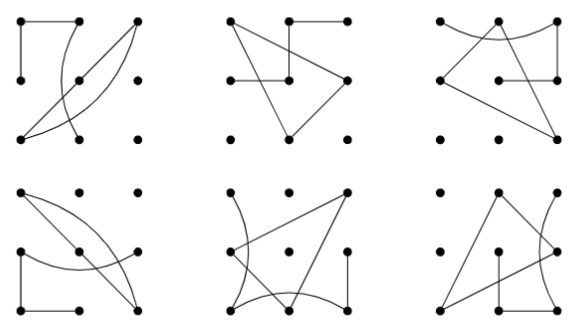
\includegraphics[scale=1.0]{K9.PNG}
\end{frame}
%%%%
\begin{frame}
\frametitle{Cyclic Designs}
\begin{itemize}
\item Let $V(K_n)=\mathbb{Z}_n$ 
\item A $G$-design is \emph{cyclic} if the permutation $v\mapsto v+1$ on $V(K_n)$ is an automorphism of the design
\item We call this \emph{clicking}
\end{itemize}
\end{frame}
%%
\begin{frame}
\frametitle{Example of a Cyclic Design}
\begin{columns}[T] % align columns
\begin{column}{.48\textwidth}
\textbf{Cyclic $P_3$-design of order 5}

\end{column}%
\hfill%
\begin{column}{.48\textwidth}
\begin{center}
    \begin{tikzpicture}[scale=0.2]
   
    
 \vertex(0) at (0,10) {0};
 \vertex(1) at (10,3) {1};
 \vertex(2) at (6,-8) {2};
 \vertex(3) at (-6,-8) {3};
 \vertex(4) at (-10,3) {4};
\tikzset{EdgeStyle/.style={}} 
%        \Edge(0)(1)
 %       \Edge(0)(3);
    \end{tikzpicture}
\end{center}
\end{column}%
\end{columns}
\end{frame}
%------------------------------------------------

\begin{frame}
\frametitle{Example of a Cyclic Design}
\begin{columns}[T] % align columns
\begin{column}{.48\textwidth}
\textbf{Cyclic $P_3$-design of order 5}\\
\color{black} $\{1,0,3\}$
\end{column}%
\hfill%
\begin{column}{.48\textwidth}
\begin{center}
    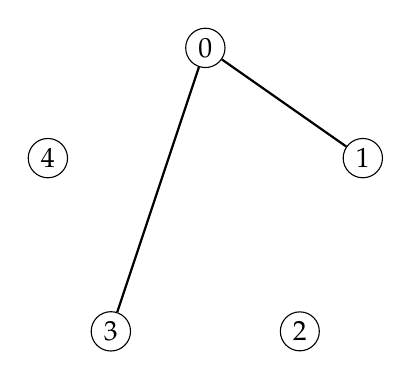
\begin{tikzpicture}[scale=0.2]
   
    
 \vertex(0) at (0,10) {0};
 \vertex(1) at (10,3) {1};
 \vertex(2) at (6,-8) {2};
 \vertex(3) at (-6,-8) {3};
 \vertex(4) at (-10,3) {4};
\tikzset{EdgeStyle/.style={}} 
        \Edge(0)(1)
        \Edge(0)(3);
    \end{tikzpicture}
\end{center}
\end{column}%
\end{columns}
\end{frame}
%--------click--------------------
\begin{frame}
\frametitle{Example of a Cyclic Design}
\begin{columns}[T] % align columns
\begin{column}{.48\textwidth}
\textbf{Cyclic $P_3$-design of order 5}\\
\color{black} $\{1,0,3\}$ \newline
\color{red} $\{2,1,4\}$
\end{column}%
\hfill%
\begin{column}{.48\textwidth}
\begin{center}
    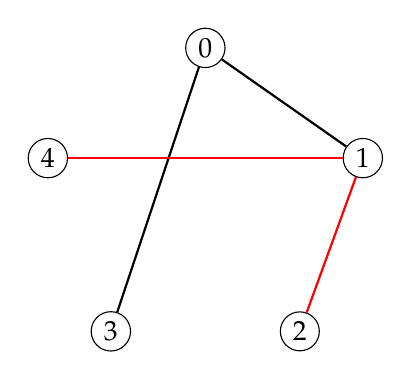
\begin{tikzpicture}[scale=0.2]
   
    
 \vertex(0) at (0,10) {0};
 \vertex(1) at (10,3) {1};
 \vertex(2) at (6,-8) {2};
 \vertex(3) at (-6,-8) {3};
 \vertex(4) at (-10,3) {4};
\tikzset{EdgeStyle/.style={}} 
        \Edge(0)(1)
        \Edge(0)(3);
\tikzset{EdgeStyle/.style={red}} 
        \Edge(4)(1)
        \Edge(1)(2);
    \end{tikzpicture}
\end{center}
\end{column}%
\end{columns}


\end{frame}
%--------click--------------------
\begin{frame}
\frametitle{Example of a Cyclic Design}
\begin{columns}[T] % align columns
\begin{column}{.48\textwidth}
\textbf{Cyclic $P_3$-design of order 5}\\
\color{black} $\{1,0,3\}$ \newline
\color{red} $\{2,1,4\}$ \newline
\color{blue}  $\{3,2,0\}$
\end{column}%
\hfill%
\begin{column}{.48\textwidth}
\begin{center}
    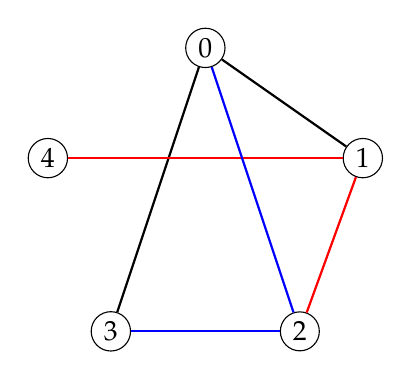
\begin{tikzpicture}[scale=0.2]
   
    
 \vertex(0) at (0,10) {0};
 \vertex(1) at (10,3) {1};
 \vertex(2) at (6,-8) {2};
 \vertex(3) at (-6,-8) {3};
 \vertex(4) at (-10,3) {4};
\tikzset{EdgeStyle/.style={}} 
        \Edge(0)(1)
        \Edge(0)(3);
\tikzset{EdgeStyle/.style={red}} 
        \Edge(4)(1)
        \Edge(1)(2);
        \tikzset{EdgeStyle/.style={blue}} 
        \Edge(0)(2)
        \Edge(3)(2);
    \end{tikzpicture}
\end{center}
\end{column}%
\end{columns}


\end{frame}

%--------click--------------------
\begin{frame}
\frametitle{Example of a Cyclic Design}
\begin{columns}[T] % align columns
\begin{column}{.48\textwidth}
\textbf{Cyclic $P_3$-design of order 5}\\
\color{black} $\{1,0,3\}$ \newline
\color{red} $\{2,1,4\}$ \newline
\color{blue} $\{3,2,0\}$\newline
\color{green}$\{4,3,1\}$
\end{column}%
\hfill%
\begin{column}{.48\textwidth}
\begin{center}
    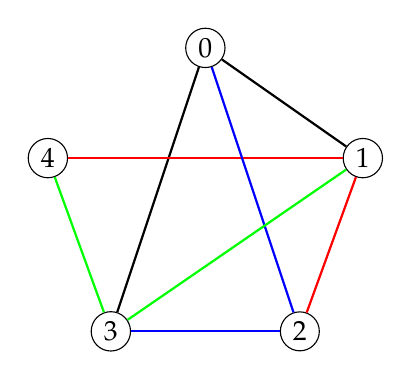
\begin{tikzpicture}[scale=0.2]
   
    
 \vertex(0) at (0,10) {0};
 \vertex(1) at (10,3) {1};
 \vertex(2) at (6,-8) {2};
 \vertex(3) at (-6,-8) {3};
 \vertex(4) at (-10,3) {4};
\tikzset{EdgeStyle/.style={}} 
        \Edge(0)(1)
        \Edge(0)(3);
\tikzset{EdgeStyle/.style={red}} 
        \Edge(4)(1)
        \Edge(1)(2);
        \tikzset{EdgeStyle/.style={blue}} 
        \Edge(0)(2)
        \Edge(3)(2);
        \tikzset{EdgeStyle/.style={green}} 
        \Edge(1)(3)
        \Edge(3)(4);
    \end{tikzpicture}
\end{center}
\end{column}%
\end{columns}


\end{frame}

%--------click--------------------
\begin{frame}
\frametitle{Example of a Cyclic Design}
\begin{columns}[T] % align columns
\begin{column}{.48\textwidth}
\textbf{Cyclic $P_3$-design of order 5}\\
\color{black} $\{1,0,3\}$ \newline
\color{red} $\{2,1,4\}$ \newline
\color{blue} $\{3,2,0\}$ \newline
\color{green} $\{4,3,1\}$\newline
\color{magenta} $\{3,2,0\}$
\end{column}%
\hfill%
\begin{column}{.48\textwidth}
\begin{center}
    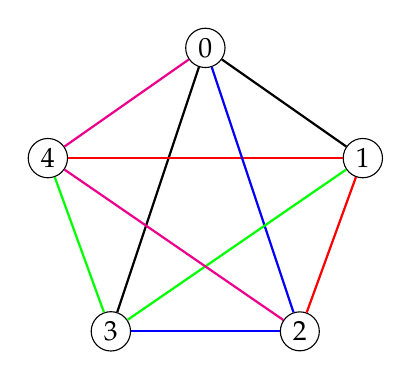
\begin{tikzpicture}[scale=0.2]
   
    
 \vertex(0) at (0,10) {0};
 \vertex(1) at (10,3) {1};
 \vertex(2) at (6,-8) {2};
 \vertex(3) at (-6,-8) {3};
 \vertex(4) at (-10,3) {4};
\tikzset{EdgeStyle/.style={}} 
        \Edge(0)(1)
        \Edge(0)(3);
\tikzset{EdgeStyle/.style={red}} 
        \Edge(4)(1)
        \Edge(1)(2);
        \tikzset{EdgeStyle/.style={blue}} 
        \Edge(0)(2)
        \Edge(3)(2);
        \tikzset{EdgeStyle/.style={green}} 
        \Edge(1)(3)
        \Edge(3)(4);
        \tikzset{EdgeStyle/.style={magenta}} 
        \Edge(2)(4)
        \Edge(0)(4);
    \end{tikzpicture}
\end{center}
\end{column}%
\end{columns}
\end{frame}
%----------------------
\section{Known Results}
%%%%%%%%%%%%%%%%%%%%%
\begin{frame}{Small Graphs}
    \begin{itemize}
        \item If $|E(G)| \leq 5,$ then the spectrum of $n$ such that a $G$-design of order $n$ exists is known
        \begin{itemize}
            \item Ex. If $G\cong C_3$, there exists a $G$-design or order $n$ (STS($n$)) iff $n \equiv 1,3 \pmod 6$
        \end{itemize}
        \pause
        \item $|E(G)|=6$
        \begin{itemize}
            \item $|V(G)|=4$ (Hanani, 1961)
            \item $|V(G)|=5$ (Bermond, Huang, Rosa, Sotteau, 1980 \& Kang, Wang, 2004)
            \item $|V(G)|=6$ (Yin, Gong, 1998)
            \item $|V(G)|=7$ (Trees: Huang, Rosa, 1978) 
            \pause
            \item \textcolor{black}{$|V(G)|\geq 7$ (Disconnected graphs)}
             \begin{itemize}
        \item \textcolor{red}{Forests (F, Peters 2023+)}
        \item \textcolor{blue}{Unicyclic graphs (Ahern, F, Froncek, Keranen, 2022+)}
    \end{itemize}
        \end{itemize}
    \end{itemize}
\end{frame}
%-----------

%%%%%%%%%%%%%%%%%%
\section{Edge Length}
%---------------------------
\begin{frame}
\frametitle{Edge Length}
\begin{itemize}
\item Let $V(K_n)=\{0,1,...,n-1\}$ 
\pause
\item The \emph{length} of edge $xy \in E(K_n)$ is min$(|x-y|,n-|x-y|)$
\pause
\item If the length of $xy$ is $n-|x-y|\geq 2,$ then $xy$ is a \emph{wrap-around} edge
\end{itemize}
\hrulefill %makes horizontal line
\pause
\begin{columns}[T] % align columns
\begin{column}{.48\textwidth}
\textbf{Edge lengths of $K_7$} \newline
\begin{itemize}
\item \color{black} length 1 \newline
%\color{blue} length 2 \newline
%\color{red} length 3 \newline
\end{itemize}
\end{column}%
\hfill%
\begin{column}{.48\textwidth}
\begin{center}
    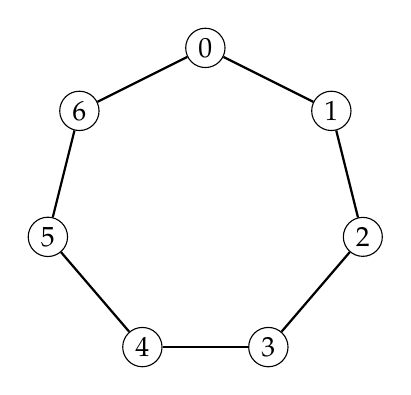
\begin{tikzpicture}[scale=0.2]
   
 \vertex(0) at (0,10) {0};
 \vertex(1) at (8,6) {1};
 \vertex(2) at (10,-2) {2};
 \vertex(3) at (4,-9) {3};
 \vertex(4) at (-4,-9) {4};
 \vertex(5) at (-10,-2) {5};
 \vertex(6) at (-8,6) {6};

\tikzset{EdgeStyle/.style={}} 
    %length 1 edges
        \Edge(0)(1)
        \Edge(1)(2)
        \Edge(2)(3)
        \Edge(3)(4)
        \Edge(4)(5)
        \Edge(5)(6)
	  \Edge(6)(0);
    \end{tikzpicture}
\end{center}
\end{column}%
\end{columns}


\end{frame}
%-------------------length 2--------------------------
\begin{frame}
\frametitle{Edge Length}
\begin{itemize}
\item Let $V(K_n)=\{0,1,...,n-1\}$ 
\item The \emph{length} of edge $xy \in E(K_n)$ is min$(|x-y|,n-|x-y|)$
\end{itemize}
\hrulefill
\begin{columns}[T] % align columns
\begin{column}{.48\textwidth}
\textbf{Edge lengths of $K_7$} \newline
\begin{itemize}
\item \color{black} length 1 \newline
\item \color{blue} length 2 \newline
%\color{red} length 3 \newline
\end{itemize}
\end{column}%
\hfill%
\begin{column}{.48\textwidth}
\begin{center}
    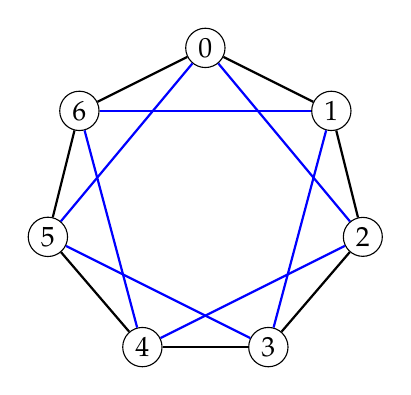
\begin{tikzpicture}[scale=0.2]
   
 \vertex(0) at (0,10) {0};
 \vertex(1) at (8,6) {1};
 \vertex(2) at (10,-2) {2};
 \vertex(3) at (4,-9) {3};
 \vertex(4) at (-4,-9) {4};
 \vertex(5) at (-10,-2) {5};
 \vertex(6) at (-8,6) {6};

\tikzset{EdgeStyle/.style={}} 
    %length 1 edges
        \Edge(0)(1)
        \Edge(1)(2)
        \Edge(2)(3)
        \Edge(3)(4)
        \Edge(4)(5)
        \Edge(5)(6)
	  \Edge(6)(0);
\tikzset{EdgeStyle/.style={blue}} 
%length 2 edges
        \Edge(0)(2)
        \Edge(2)(4)
        \Edge(4)(6)
        \Edge(6)(1)
        \Edge(3)(5)
        \Edge(3)(1)
        \Edge(5)(0);

    \end{tikzpicture}
\end{center}
\end{column}%
\end{columns}


\end{frame}
%---------------length 3-----------------
\begin{frame}
\frametitle{Edge Length}
\begin{itemize}
\item Let $V(K_n)=\{0,1,...,n-1\}$ 
\item The \emph{length} of edge $xy \in E(K_n)$ is min$(|x-y|,n-|x-y|)$
\end{itemize}
\hrulefill
\begin{columns}[T] % align columns
\begin{column}{.48\textwidth}
\textbf{Edge lengths of $K_7$} \newline
\begin{itemize}
\item \color{black} length 1 \newline
\item \color{blue} length 2 \newline
\item \color{red} length 3 \newline
\end{itemize}
\end{column}%
\hfill%
\begin{column}{.48\textwidth}
\begin{center}
    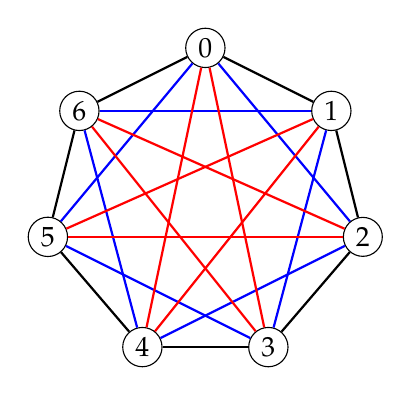
\begin{tikzpicture}[scale=0.2]
   
 \vertex(0) at (0,10) {0};
 \vertex(1) at (8,6) {1};
 \vertex(2) at (10,-2) {2};
 \vertex(3) at (4,-9) {3};
 \vertex(4) at (-4,-9) {4};
 \vertex(5) at (-10,-2) {5};
 \vertex(6) at (-8,6) {6};

\tikzset{EdgeStyle/.style={}} 
    %length 1 edges
        \Edge(0)(1)
        \Edge(1)(2)
        \Edge(2)(3)
        \Edge(3)(4)
        \Edge(4)(5)
        \Edge(5)(6)
	  \Edge(6)(0);
\tikzset{EdgeStyle/.style={blue}} 
%length 2 edges
        \Edge(0)(2)
        \Edge(2)(4)
        \Edge(4)(6)
        \Edge(6)(1)
        \Edge(3)(5)
        \Edge(3)(1)
        \Edge(5)(0);
\tikzset{EdgeStyle/.style={red}} 
%length 3 edges
        \Edge(0)(3)
        \Edge(3)(6)
        \Edge(6)(2)
        \Edge(2)(5)
        \Edge(1)(5)
        \Edge(1)(4)
         \Edge(4)(0);

    \end{tikzpicture}
\end{center}
\end{column}%
\end{columns}


\end{frame}
%--------------edge length and cyclic decomp---
\begin{frame}
\frametitle{Edge Length and Cyclic Decomposition}
\begin{itemize}
    \item Notice that edge length is preserved by the permutation $v\mapsto v+1$ on $V(K_n)$
    \pause
    \item Also, when $n$ is odd, edge length partitions $E(K_n)$ into $\frac{n-1}{2}$ (the number of lengths) sets of size $n$ (the number of edges of each length) 
    \pause
\end{itemize}
\begin{center}
    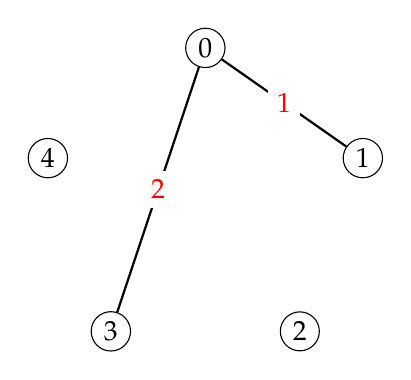
\begin{tikzpicture}[scale=0.2]
   
    
 \vertex(0) at (0,10) {0};
 \vertex(1) at (10,3) {1};
 \vertex(2) at (6,-8) {2};
 \vertex(3) at (-6,-8) {3};
 \vertex(4) at (-10,3) {4};
\tikzset{EdgeStyle/.style={}} 
        \Edge[label=\textcolor{red}{1}](0)(1)
        \Edge[label=\textcolor{red}{2}](0)(3);

    \end{tikzpicture}
\end{center}
    
\end{frame}
%-----------click-----
\begin{frame}
\frametitle{Edge Length and Cyclic Decomposition}
\begin{itemize}
    \item Notice that edge length is preserved by the permutation $v\mapsto v+1$ on $V(K_n)$
    \item Also, when $n$ is odd, edge length partitions $E(K_n)$ into $\frac{n-1}{2}$ (the number of lengths) sets of size $n$ (the number of edges of each length) 
\end{itemize}
\begin{center}
    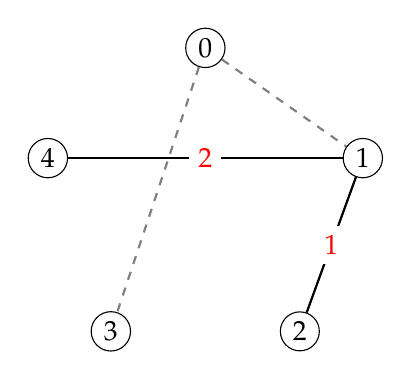
\begin{tikzpicture}[scale=0.2]
   
    
 \vertex(0) at (0,10) {0};
 \vertex(1) at (10,3) {1};
 \vertex(2) at (6,-8) {2};
 \vertex(3) at (-6,-8) {3};
 \vertex(4) at (-10,3) {4};
\tikzset{EdgeStyle/.style={dashed, gray}} 
        \Edge(0)(1)
        \Edge(0)(3);
        \tikzset{EdgeStyle/.style={}} 
        \Edge[label=\textcolor{red}{2}](4)(1)
        \Edge[label=\textcolor{red}{1}](1)(2);
      
    \end{tikzpicture}
\end{center}
    
\end{frame}
%-click---------------
\begin{frame}
\frametitle{Edge Length and Cyclic Decomposition}
\begin{itemize}
    \item Notice that edge length is preserved by the permutation $v\mapsto v+1$ on $V(K_n)$
    \item Also, when $n$ is odd, edge length partitions $E(K_n)$ into $\frac{n-1}{2}$ (the number of lengths) sets of size $n$ (the number of edges of each length) 
\end{itemize}
\begin{center}
    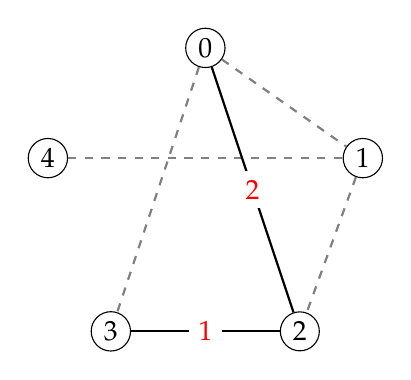
\begin{tikzpicture}[scale=0.2]
   
    
 \vertex(0) at (0,10) {0};
 \vertex(1) at (10,3) {1};
 \vertex(2) at (6,-8) {2};
 \vertex(3) at (-6,-8) {3};
 \vertex(4) at (-10,3) {4};
\tikzset{EdgeStyle/.style={dashed, gray}} 
        \Edge(0)(1)
        \Edge(0)(3);
\tikzset{EdgeStyle/.style={dashed, gray}} 
        \Edge(4)(1)
        \Edge(1)(2);
\tikzset{EdgeStyle/.style={}} 
        \Edge[label=\textcolor{red}{2}](0)(2)
        \Edge[label=\textcolor{red}{1}](3)(2);
      
    \end{tikzpicture}
\end{center}
    
\end{frame}
%---click-----------
\begin{frame}
\frametitle{Edge Length and Cyclic Decomposition}
\begin{itemize}
    \item Notice that edge length is preserved by the permutation $v\mapsto v+1$ on $V(K_n)$
    \item Also, when $n$ is odd, edge length partitions $E(K_n)$ into $\frac{n-1}{2}$ (the number of lengths) sets of size $n$ (the number of edges of each length) 
\end{itemize}
\begin{center}
    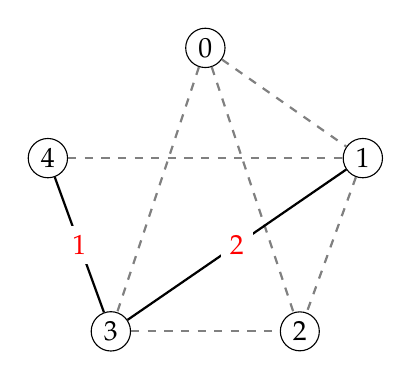
\begin{tikzpicture}[scale=0.2]
   
    
 \vertex(0) at (0,10) {0};
 \vertex(1) at (10,3) {1};
 \vertex(2) at (6,-8) {2};
 \vertex(3) at (-6,-8) {3};
 \vertex(4) at (-10,3) {4};
\tikzset{EdgeStyle/.style={dashed, gray}} 
        \Edge(0)(1)
        \Edge(0)(3);
\tikzset{EdgeStyle/.style={dashed, gray}} 
        \Edge(4)(1)
        \Edge(1)(2);
 \tikzset{EdgeStyle/.style={dashed, gray}}       
        \Edge(0)(2)
        \Edge(3)(2);
\tikzset{EdgeStyle/.style={}}         
        \Edge[label=\textcolor{red}{2}](1)(3)
        \Edge[label=\textcolor{red}{1}](3)(4);
      
    \end{tikzpicture}
\end{center}
    
\end{frame}

%----click------
\begin{frame}
\frametitle{Edge Length and Cyclic Decomposition}
\begin{itemize}
    \item Notice that edge length is preserved by the permutation $v\mapsto v+1$ on $V(K_n)$
    \item Also, when $n$ is odd, edge length partitions $E(K_n)$ into $\frac{n-1}{2}$ (the number of lengths) sets of size $n$ (the number of edges of each length) 
\end{itemize}
\begin{center}
    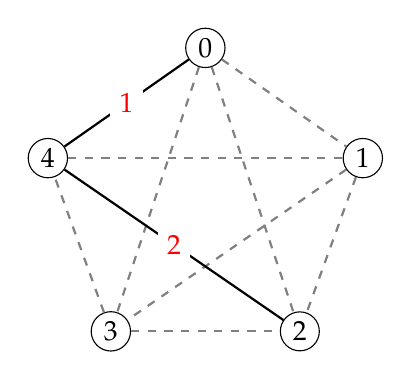
\begin{tikzpicture}[scale=0.2]
   
    
 \vertex(0) at (0,10) {0};
 \vertex(1) at (10,3) {1};
 \vertex(2) at (6,-8) {2};
 \vertex(3) at (-6,-8) {3};
 \vertex(4) at (-10,3) {4};
\tikzset{EdgeStyle/.style={dashed, gray}} 
        \Edge(0)(1)
        \Edge(0)(3);
\tikzset{EdgeStyle/.style={dashed, gray}} 
        \Edge(4)(1)
        \Edge(1)(2);
   \tikzset{EdgeStyle/.style={dashed, gray}}    
        \Edge(0)(2)
        \Edge(3)(2);
 \tikzset{EdgeStyle/.style={dashed, gray}}     
        \Edge(1)(3)
        \Edge(3)(4);
 \tikzset{EdgeStyle/.style={}}    
        \Edge[label=\textcolor{red}{2}](2)(4)
        \Edge[label=\textcolor{red}{1}](0)(4);
    \end{tikzpicture}
\end{center}
    
\end{frame}
%----click------
\begin{frame}
\frametitle{Edge Length and Cyclic Decomposition}
\begin{itemize}
    \item Notice that edge length is preserved by the permutation $v\mapsto v+1$ on $V(K_n)$
    \item Also, when $n$ is odd, edge length partitions $E(K_n)$ into $\frac{n-1}{2}$ (the number of lengths) sets of size $n$ (the number of edges of each length) 
\end{itemize}
\begin{center}
    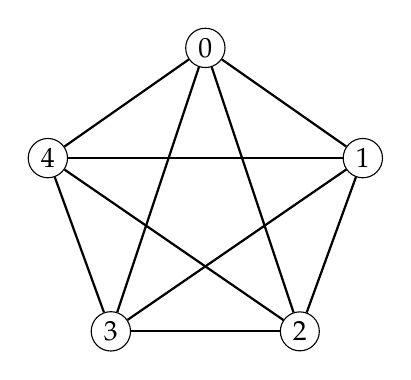
\begin{tikzpicture}[scale=0.2]
   
    
 \vertex(0) at (0,10) {0};
 \vertex(1) at (10,3) {1};
 \vertex(2) at (6,-8) {2};
 \vertex(3) at (-6,-8) {3};
 \vertex(4) at (-10,3) {4};
\tikzset{EdgeStyle/.style={}} 
        \Edge(0)(1)
        \Edge(0)(3);
\tikzset{EdgeStyle/.style={}} 
        \Edge(4)(1)
        \Edge(1)(2);
   \tikzset{EdgeStyle/.style={}}    
        \Edge(0)(2)
        \Edge(3)(2);
 \tikzset{EdgeStyle/.style={}}     
        \Edge(1)(3)
        \Edge(3)(4);
 \tikzset{EdgeStyle/.style={}}    
        \Edge(2)(4)
        \Edge(0)(4);
    \end{tikzpicture}
\end{center}
    
\end{frame}
%---------------------------------
%%%%%%%%%%%%%%%%%%%%%%%%%%%%%%%%%
%%%%%%%%%%%%%%%%%%%%%%%%%%%%%
\section{Rosa-type Labelings}

%--------------rho defn and exmpl-------------
\begin{frame}
\frametitle{Rosa-type Labelings}
\begin{block}{$\rho$-labeling}
Let $G$ be a simple graph with $n$ edges. A $\rho$-\emph{labeling} of $G$ is a one-to-one function $f:V(G) \rightarrow \{0,1,...,2n\}$ such that the set of induced edge lengths is $\{1,2,...,n\}.$
\end{block}
\begin{center}
    \begin{tikzpicture}[scale=0.3]
 \vertex(0) at (0,0) {0};
 \vertex(1) at (10,0) {1};
\vertex(3) at (20,0) {3};
\vertex(6) at (30,0) {6};
\vertex (7) at (20,10) {7};
        \Edge(0)(1) ;
        \Edge(1)(3);
        \Edge(6)(3);
        \Edge(3)(7);    
    \end{tikzpicture}
\end{center}

\end{frame}
%--------------show edge lengths----------------
\begin{frame}
\frametitle{Rosa-type Labelings}
\begin{block}{$\rho$-labeling}
Let $G$ be a simple graph with $n$ edges. A $\rho$-\emph{labeling} of $G$ is a one-to-one function $f:V(G) \rightarrow \{0,1,...,2n\}$ such that the set of induced edge lengths is $\{1,2,...,n\}.$
\end{block}
\begin{center}
    \begin{tikzpicture}[scale=0.3]
 \vertex(0) at (0,0) {0};
 \vertex(1) at (10,0) {1};
\vertex(3) at (20,0) {3};
\vertex(6) at (30,0) {6};
\vertex (7) at (20,10) {7};
        \Edge[label=\textcolor{blue}{1}](0)(1) ;
        \Edge[label=\textcolor{blue}{2}](1)(3);
        \Edge[label=\textcolor{blue}{3}](6)(3);
        \Edge[label=\textcolor{blue}{4}](3)(7);
    \end{tikzpicture}
\end{center}
\end{frame}
%---------------

\begin{frame}
\frametitle{Rosa-type Labelings}
\begin{block}{$\rho$-labeling}
Let $G$ be a simple graph with $n$ edges. A $\rho$-\emph{labeling} of $G$ is a one-to-one function $f:V(G) \rightarrow \{0,1,...,2n\}$ such that the set of induced edge lengths is $\{1,2,...,n\}.$
\end{block}
\begin{theorem}[Rosa, 1967]
Let $G$ be a graph with $n$ edges. A cyclic decomposition of $K_{2n+1}$ exists if and only if $G$ admits a $\rho$-labeling.
\end{theorem}
\end{frame}
%%-----------------rho plus -----------

\begin{frame}
\frametitle{Rosa-type Labelings}
\begin{block}{Ordered $\rho$-labeling}
A $\rho$-labeling of a bipartite graph $G$ with bipartition $(\textcolor{blue}{X},\textcolor{red}{Y})$ is called an \emph{ordered} $\rho$-labeling and denoted $\rho^+$, if $\textcolor{blue}{f(x)}<\textcolor{red}{f(y)}$ for each edge $xy$ with \textcolor{blue}{$x\in X$} and \textcolor{red}{$y \in Y$}.
\end{block}
\begin{center}
    \begin{tikzpicture}[scale=0.3]
 \vertex(0) at (0,0) {\textcolor{blue}{1}};
 \vertex(1) at (10,0) {\textcolor{red}{2}};
\vertex(3) at (20,0) {\textcolor{blue}{0}};
\vertex(6) at (30,0) {\textcolor{red}{4}};
\vertex (7) at (20,10) {\textcolor{red}{3}};
        \Edge[label=1](0)(1) ;
        \Edge[label=2](1)(3);
        \Edge[label=4](6)(3);
        \Edge[label=3](3)(7);
    \end{tikzpicture}
\end{center}
\end{frame}
%-----------------------------
\begin{frame}
\frametitle{Rosa-type Labelings}
\begin{block}{Ordered $\rho$-labeling}
A $\rho$-labeling of a bipartite graph $G$ with bipartition $(\textcolor{blue}{X},\textcolor{red}{Y})$ is called an \emph{ordered} $\rho$-labeling and denoted $\rho^+$, if $\textcolor{blue}{f(x)}<\textcolor{red}{f(y)}$ for each edge $xy$ with \textcolor{blue}{$x\in X$} and \textcolor{red}{$y \in Y$}.
\end{block}
\begin{theorem}[El-Zanati, Vanden Eynden, Punnim, 2001]
Let $G$ be a graph with $n$ edges which has a $\rho^+$ labeling. Then $G$ decomposes $K_{2nt+1}$ for all positive integers $t.$
\end{theorem}
\pause
\begin{center}
    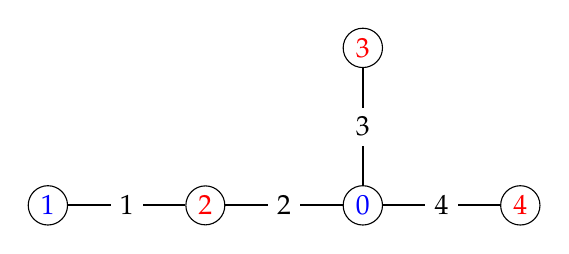
\begin{tikzpicture}[scale=0.2]
 \vertex(0) at (0,0) {\textcolor{blue}{1}};
 \vertex(1) at (10,0) {\textcolor{red}{2}};
\vertex(3) at (20,0) {\textcolor{blue}{0}};
\vertex(6) at (30,0) {\textcolor{red}{4}};
\vertex (7) at (20,10) {\textcolor{red}{3}};
        \Edge[label=1](0)(1) ;
        \Edge[label=2](1)(3);
        \Edge[label=4](6)(3);
        \Edge[label=3](3)(7);
    \end{tikzpicture}
\end{center}
\end{frame}
%-----rho tripartite----------
\begin{frame}
\frametitle{Tripartite Graphs}
\begin{itemize}
\item Bunge, Chantasartrassmee, El-Zanati, and Vanden Eynden introduced the following in 2013.
\pause
\item Let $G$ be a tripartite graph with $n$ edges and vertex tripartition $\{A,B,C\}$. A $\rho$-\emph{tripartite labeling} of $G$ is a $\rho$-labeling $f$ that satisfies the following conditions.\pause
\begin{enumerate}
\item $f(a)<f(v)$ for every edge $av$ with $a \in A.$
\item For every edge $bc$ with $b \in B$ and $c \in C,$ there exists a complementary edge $b'c'$ with $b' \in B$ and $c' \in C$ such that 
\[ |f(b)-f(c)|+|f(b')-f(c')|=2n.
\]
\item For all $b \in B$ and $c \in C$, we have
\[|f(b)-f(c)| \neq 2n.
\]
\end{enumerate}
\end{itemize}


\end{frame}
%-------------def with pic
\begin{frame}{Example}
    
Let $G$ be a tripartite graph with $n$ edges and vertex tripartition $\{\textcolor{green}{A},\textcolor{blue}{B},\textcolor{red}{C}\}$. A $\rho$-\emph{tripartite labeling} of $G$ is a $\rho$-labeling $f$ that satisfies the following conditions.
\begin{enumerate}
\item $\textcolor{green}{f(a)}<f(v)$ for every edge $av$ with $a \in A.$
\item For every edge $bc$ with $b \in B$ and $c \in C,$ there exists a complementary edge $b'c'$ with $b' \in B$ and $c' \in C$ such that 
$ |\textcolor{blue}{f(b)}-\textcolor{red}{f(c)}|+|\textcolor{blue}{f(b')}-\textcolor{red}{f(c')}|=2n.$
\item $|\textcolor{blue}{f(b)}-\textcolor{red}{f(c)}| \neq 2n$ or all $b \in B$ and $c \in C$.
\end{enumerate}
\begin{center}
    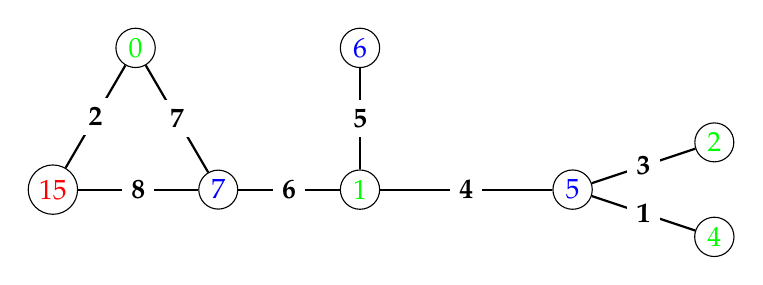
\begin{tikzpicture}[scale=0.3]
   \tikzstyle{vertex}=[circle, draw, inner sep=2pt, minimum size=10pt]
    
 \vertex(1) at (0,0) {\textcolor{red}{15}};
 \vertex(2) at (3.5,6) {\textcolor{green}{0}};
 \vertex(3) at (7,0) {\textcolor{blue}{7}};
 \vertex(4) at (13,0) {\textcolor{green}{1}};
 \vertex(5) at (13,6) {\textcolor{blue}{6}};
\vertex(6) at (22,0) {\textcolor{blue}{5}};
 \vertex(7) at (28,-2) {\textcolor{green}{4}};
 \vertex(8) at (28,2) {\textcolor{green}{2}};
\tikzset{EdgeStyle/.style={}} % insert --> in brackets for directed graph or bend right etc
        \Edge[label=\bf{2}](1)(2)
        \Edge[label=\bf{8}](1)(3)
        \Edge[label=\bf{7}](3)(2)
        \Edge[label=\bf{6}](4)(3)
        \Edge[label=\bf{5}](5)(4)
        \Edge[label=\bf{4}](4)(6)
        \Edge[label=\bf{1}](6)(7)
        \Edge[label=\bf{3}](6)(8);
    \end{tikzpicture}
\end{center}
\end{frame}

%--------Bunge et al thm and pic
\begin{frame}
\frametitle{Tripartite Graphs }
\begin{theorem}[Bunge et al., 2013]
Let $G$ be a tripartite graph on $n$ edges which admits a $\rho$-tripartite labeling. Then there exists a cyclic $G$-decomposition of $K_{2nt+1}$ for all $t\geq 1.$
\end{theorem}
\begin{center}
    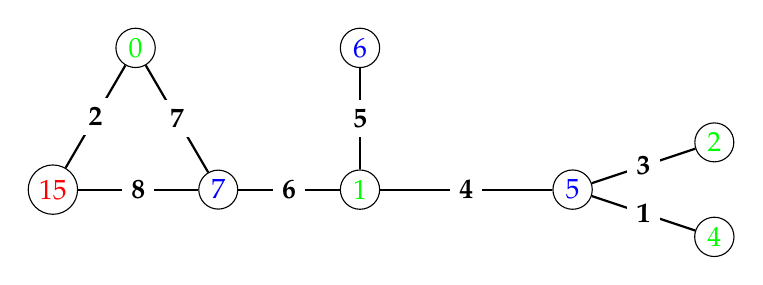
\begin{tikzpicture}[scale=0.3]
   \tikzstyle{vertex}=[circle, draw, inner sep=2pt, minimum size=10pt]
    
 \vertex(1) at (0,0) {\textcolor{red}{15}};
 \vertex(2) at (3.5,6) {\textcolor{green}{0}};
 \vertex(3) at (7,0) {\textcolor{blue}{7}};
 \vertex(4) at (13,0) {\textcolor{green}{1}};
 \vertex(5) at (13,6) {\textcolor{blue}{6}};
\vertex(6) at (22,0) {\textcolor{blue}{5}};
 \vertex(7) at (28,-2) {\textcolor{green}{4}};
 \vertex(8) at (28,2) {\textcolor{green}{2}};
\tikzset{EdgeStyle/.style={}} % insert --> in brackets for directed graph or bend right etc
        \Edge[label=\bf{2}](1)(2)
        \Edge[label=\bf{8}](1)(3)
        \Edge[label=\bf{7}](3)(2)
        \Edge[label=\bf{6}](4)(3)
        \Edge[label=\bf{5}](5)(4)
        \Edge[label=\bf{4}](4)(6)
        \Edge[label=\bf{1}](6)(7)
        \Edge[label=\bf{3}](6)(8);
    \end{tikzpicture}
\end{center}
\end{frame}
%---------------
\begin{frame}{$1$-Rotational Designs}
    Can we take a similar approach when $n$ is even?
    \begin{columns}[T] % align columns
\begin{column}{.48\textwidth}
 \begin{center}
    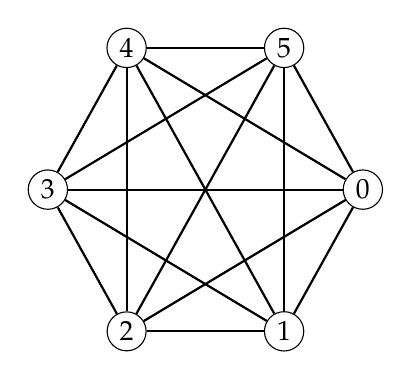
\begin{tikzpicture}[scale=0.2]
   \tikzstyle{vertex}=[circle, draw, inner sep=2pt, minimum size=10pt]
   

 \vertex(1) at (10,0) {0};
 \vertex(2) at (5,-9) {1};
 \vertex(3) at (-10,0) {3};
 \vertex(4) at (-5,9) {4};
 \vertex(5) at (5,9) {5};
\vertex(6) at (-5,-9) {2};

\tikzset{EdgeStyle/.style={}} % insert --> in brackets for directed graph or bend right etc
        \Edge[](1)(2)
        \Edge[](1)(3)
        \Edge[](1)(4)
        \Edge[](1)(5)
        \Edge[](1)(6)
        \Edge[](2)(3)
        \Edge[](2)(4)
        \Edge[](2)(5)
        \Edge[](2)(6)
        \Edge[](3)(4)
        \Edge[](3)(5)
        \Edge[](3)(6)
        \Edge[](4)(5)
        \Edge[](4)(6)
        \Edge[](5)(6);
      
    \end{tikzpicture}
\end{center}
\end{column}%
\hfill%
\pause
\begin{column}{.48\textwidth}
\begin{center}
    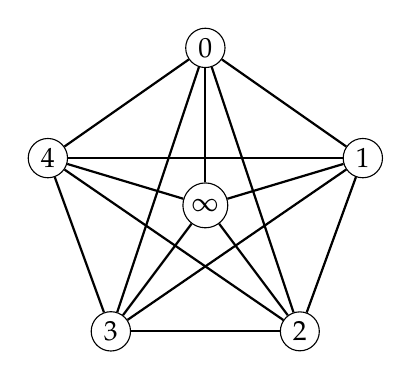
\begin{tikzpicture}[scale=0.2]
 
 \vertex(0) at (0,10) {0};
 \vertex(1) at (10,3) {1};
 \vertex(2) at (6,-8) {2};
 \vertex(3) at (-6,-8) {3};
 \vertex(4) at (-10,3) {4};
\vertex(5) at (0,0) {$\infty$};
\tikzset{EdgeStyle/.style={}} 
        \Edge(0)(1)
        \Edge(0)(2)
        \Edge(0)(3)
        \Edge(0)(4)
        \Edge(0)(5)
        \Edge(1)(2)
        \Edge(1)(3)
        \Edge(1)(4)
        \Edge(2)(3)
        \Edge(2)(4)
        \Edge(3)(4)
        \Edge(5)(1)
        \Edge(5)(2)
        \Edge(5)(3)
        \Edge(5)(4);
    \end{tikzpicture}
\end{center}
\end{column}%
\end{columns}
\end{frame}
%%%%-----definition 1-rot 
%-------1-rotational----

\begin{frame}
\frametitle{1-Rotational Designs}
\begin{itemize}
\item Let $V(K_{2n})=\{0,1,2,...,2n-2,\infty\}$
and $G$ be a graph with $n$ edges and at least one pendant edge.
\end{itemize}
\pause
\begin{block}{1-rotational $\rho$-labeling}
A \emph{1-rotational $\rho$-labeling} of $G$ is an embedding of $G$ into $K_{2n}$ such that the edge lengths form the set $\{1,2,...,n-1,\infty\}.$
\end{block}
\pause
\begin{columns}[T] % align columns
\begin{column}{.48\textwidth}
\textbf{A 1-rotational $P_{4}$-design of order 6}
\end{column}%
\hfill%
\begin{column}{.48\textwidth}
\begin{center}
    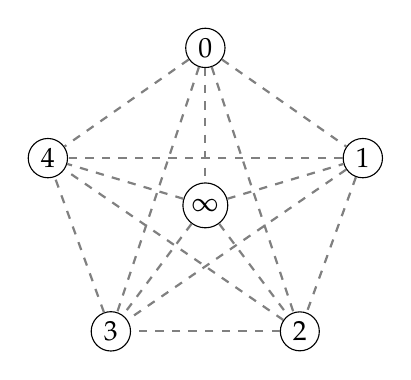
\begin{tikzpicture}[scale=0.2]
 \vertex(0) at (0,10) {0};
 \vertex(1) at (10,3) {1};
 \vertex(2) at (6,-8) {2};
 \vertex(3) at (-6,-8) {3};
 \vertex(4) at (-10,3) {4};
\vertex(5) at (0,0) {$\infty$};
\tikzset{EdgeStyle/.style={dashed,gray}} 
         \Edge(0)(1)
        \Edge(0)(2)
        \Edge(0)(3)
        \Edge(0)(4)
        \Edge(0)(5)
        \Edge(1)(2)
        \Edge(1)(3)
        \Edge(1)(4)
        \Edge(2)(3)
        \Edge(2)(4)
        \Edge(3)(4)
        \Edge(5)(1)
        \Edge(5)(2)
        \Edge(5)(3)
        \Edge(5)(4);
    \end{tikzpicture}

\end{center}
\end{column}%
\end{columns}

\end{frame}
%--------click 1---------
\begin{frame}
\frametitle{1-Rotational Designs}
\begin{itemize}
\item Let $V(K_{2n})=\{0,1,2,...,2n-2,\infty\}.$\\

\item Let $G$ be a graph with $n$ edges and at least one pendant edge.
\end{itemize}

\begin{block}{1-rotational $\rho$-labeling}
A \emph{1-rotational $\rho$-labeling} of $G$ is an embedding of $G$ into $K_{2n}$ such that the edge lengths form the set $\{1,2,...,n-1,\infty\}.$
\end{block}

\begin{columns}[T] % align columns
\begin{column}{.48\textwidth}
\textbf{A 1-rotational $P_{4}$-design of order 6}
\begin{itemize}
\item \color{black} $(0,2,1,\infty)$ 
%\item \color{blue} $(1,3,2,\infty)$ \newline
%\item \color{red} $(2,4,3,\infty)$ \newline
%\item \color{green} $(3,0,4,\infty)$ \newline
%\item \color{magenta} $(4,1,0,\infty)$ \newline

\end{itemize}
\end{column}%
\hfill%
\begin{column}{.48\textwidth}
\begin{center}
    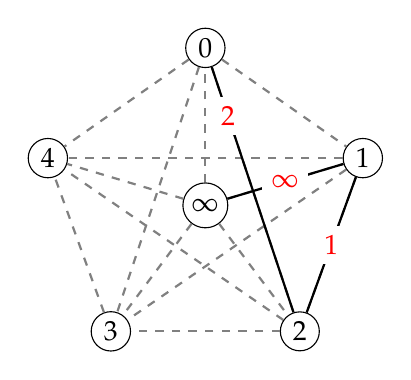
\begin{tikzpicture}[scale=0.2]
 
 \vertex(0) at (0,10) {0};
 \vertex(1) at (10,3) {1};
 \vertex(2) at (6,-8) {2};
 \vertex(3) at (-6,-8) {3};
 \vertex(4) at (-10,3) {4};
\vertex(5) at (0,0) {$\infty$};
\tikzset{EdgeStyle/.style={dashed,gray}} 
        \Edge(0)(1)
        \Edge(0)(2);
        \Edge(0)(3)
        \Edge(0)(4);
        \Edge(1)(2)
        \Edge(1)(3);
        \Edge(1)(4)
        \Edge(2)(3);
        \Edge(2)(4)
        \Edge(3)(4);
        \Edge(5)(0)
        \Edge(5)(1)
        \Edge(5)(2)
        \Edge(5)(3)
        \Edge(5)(4);
        %click
        \tikzset{EdgeStyle/.style={black}}
        
      
      \Edge[label=\textcolor{red}{2},style={pos=0.2}](0)(2)
        
       \Edge[label=\textcolor{red}{1}](2)(1)
        \Edge[label=\textcolor{red}{$\infty$}](1)(5);
    \end{tikzpicture}

\end{center}
\end{column}%
\end{columns}

\end{frame}
%--------click 2---------
\begin{frame}
\frametitle{1-Rotational Designs}
\begin{itemize}
\item Let $V(K_{2n})=\{0,1,2,...,2n-2,\infty\}.$\\

\item Let $G$ be a graph with $n$ edges and at least one pendant edge.
\end{itemize}

\begin{block}{1-rotational $\rho$-labeling}
A \emph{1-rotational $\rho$-labeling} of $G$ is an embedding of $G$ into $K_{2n}$ such that the edge lengths form the set $\{1,2,...,n-1,\infty\}.$
\end{block}

\begin{columns}[T] % align columns
\begin{column}{.48\textwidth}
\textbf{A 1-rotational $P_{4}$-design of order 6}
\begin{itemize}
\item \color{black} $(0,2,1,\infty)$ 
\item \color{blue} $(1,3,2,\infty)$ 
%\item \color{red} $(2,4,3,\infty)$ \newline
%\item \color{green} $(3,0,4,\infty)$ \newline
%\item \color{magenta} $(4,1,0,\infty)$ \newline

\end{itemize}
\end{column}%
\hfill%
\begin{column}{.48\textwidth}
\begin{center}
    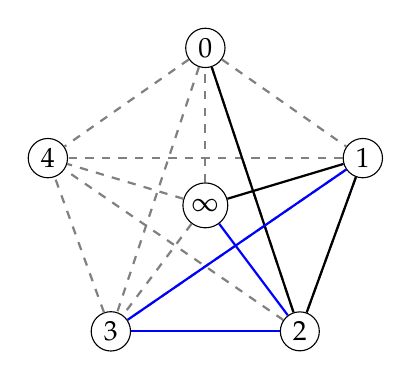
\begin{tikzpicture}[scale=0.2]
 
 \vertex(0) at (0,10) {0};
 \vertex(1) at (10,3) {1};
 \vertex(2) at (6,-8) {2};
 \vertex(3) at (-6,-8) {3};
 \vertex(4) at (-10,3) {4};
\vertex(5) at (0,0) {$\infty$};
\tikzset{EdgeStyle/.style={dashed,gray}} 
        \Edge(0)(1)
        \Edge(0)(2);
        \Edge(0)(3)
        \Edge(0)(4);
        \Edge(1)(2)
        \Edge(1)(3);
        \Edge(1)(4)
        \Edge(2)(3);
        \Edge(2)(4)
        \Edge(3)(4);
        \Edge(5)(3)
        \Edge(5)(4)
        \Edge(5)(0);
        %click
        \tikzset{EdgeStyle/.style={black}}
      \Edge(0)(2)
        \Edge(2)(1)
        \Edge(1)(5);
        
         \tikzset{EdgeStyle/.style={blue}}
      \Edge(1)(3)
        \Edge(2)(3)
        \Edge(2)(5);
    \end{tikzpicture}

\end{center}
\end{column}%
\end{columns}

\end{frame}
%--------click 3---------
\begin{frame}
\frametitle{1-Rotational Designs}
\begin{itemize}
\item Let $V(K_{2n})=\{0,1,2,...,2n-2,\infty\}.$\\

\item Let $G$ be a graph with $n$ edges and at least one pendant edge.
\end{itemize}

\begin{block}{1-rotational $\rho$-labeling}
A \emph{1-rotational $\rho$-labeling} of $G$ is an embedding of $G$ into $K_{2n}$ such that the edge lengths form the set $\{1,2,...,n-1,\infty\}.$
\end{block}

\begin{columns}[T] % align columns
\begin{column}{.48\textwidth}
\textbf{A 1-rotational $P_{4}$-design of order 6}
\begin{itemize}
\item \color{black} $(0,2,1,\infty)$ 
\item \color{blue} $(1,3,2,\infty)$ 
\item \color{red} $(2,4,3,\infty)$ 
%\item \color{green} $(3,0,4,\infty)$ \newline
%\item \color{magenta} $(4,1,0,\infty)$ \newline

\end{itemize}
\end{column}%
\hfill%
\begin{column}{.48\textwidth}
\begin{center}
    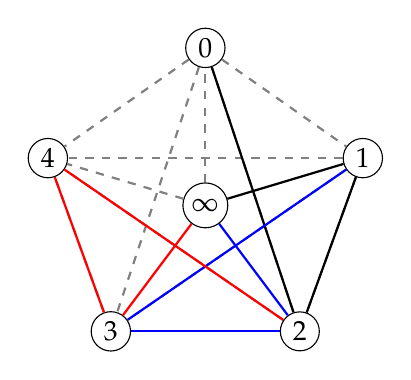
\begin{tikzpicture}[scale=0.2]
 
 \vertex(0) at (0,10) {0};
 \vertex(1) at (10,3) {1};
 \vertex(2) at (6,-8) {2};
 \vertex(3) at (-6,-8) {3};
 \vertex(4) at (-10,3) {4};
\vertex(5) at (0,0) {$\infty$};
\tikzset{EdgeStyle/.style={dashed,gray}} 
        \Edge(0)(1)
        \Edge(0)(2);
        \Edge(0)(3)
        \Edge(0)(4);
        \Edge(1)(2)
        \Edge(1)(3);
        \Edge(1)(4)
        \Edge(2)(3);
        \Edge(2)(4)
        \Edge(5)(4)
        \Edge(5)(0)
        \Edge(3)(4);
        \tikzset{EdgeStyle/.style={black}}
      \Edge(0)(2)
        \Edge(2)(1)
        \Edge(1)(5);
        
         \tikzset{EdgeStyle/.style={blue}}
      \Edge(1)(3)
        \Edge(2)(3)
        \Edge(2)(5);
        
        \tikzset{EdgeStyle/.style={red}}
      \Edge(2)(4)
        \Edge(4)(3)
        \Edge(3)(5);
    \end{tikzpicture}

\end{center}
\end{column}%
\end{columns}

\end{frame}
%--------click 4---------
\begin{frame}
\frametitle{1-Rotational Designs}
\begin{itemize}
\item Let $V(K_{2n})=\{0,1,2,...,2n-2,\infty\}.$\\

\item Let $G$ be a graph with $n$ edges and at least one pendant edge.
\end{itemize}

\begin{block}{1-rotational $\rho$-labeling}
A \emph{1-rotational $\rho$-labeling} of $G$ is an embedding of $G$ into $K_{2n}$ such that the edge lengths form the set $\{1,2,...,n-1,\infty\}.$
\end{block}

\begin{columns}[T] % align columns
\begin{column}{.48\textwidth}
\textbf{A 1-rotational $P_{4}$-design of order 6}
\begin{itemize}
\item \color{black} $(0,2,1,\infty)$ 
\item \color{blue} $(1,3,2,\infty)$ 
\item \color{red} $(2,4,3,\infty)$ 
\item \color{green} $(3,0,4,\infty)$ 
%\item \color{magenta} $(4,1,0,\infty)$ \newline

\end{itemize}
\end{column}%
\hfill%
\begin{column}{.48\textwidth}
\begin{center}
    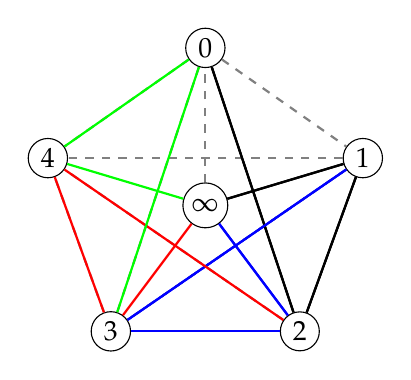
\begin{tikzpicture}[scale=0.2]
 
 \vertex(0) at (0,10) {0};
 \vertex(1) at (10,3) {1};
 \vertex(2) at (6,-8) {2};
 \vertex(3) at (-6,-8) {3};
 \vertex(4) at (-10,3) {4};
\vertex(5) at (0,0) {$\infty$};
\tikzset{EdgeStyle/.style={dashed,gray}} 
        \Edge(0)(1)
        \Edge(0)(2);
        \Edge(0)(3)
        \Edge(0)(4);
        \Edge(1)(2)
        \Edge(1)(3);
        \Edge(1)(4)
        \Edge(2)(3);
        \Edge(2)(4)
        \Edge(5)(0)
        \Edge(3)(4);
       \tikzset{EdgeStyle/.style={black}}
      \Edge(0)(2)
        \Edge(2)(1)
        \Edge(1)(5);
        
         \tikzset{EdgeStyle/.style={blue}}
      \Edge(1)(3)
        \Edge(2)(3)
        \Edge(2)(5);
        
         \tikzset{EdgeStyle/.style={black}}
      \Edge(0)(2)
        \Edge(2)(1)
        \Edge(1)(5);
        
         \tikzset{EdgeStyle/.style={blue}}
      \Edge(1)(3)
        \Edge(2)(3)
        \Edge(2)(5);
        
        \tikzset{EdgeStyle/.style={red}}
      \Edge(2)(4)
        \Edge(4)(3)
        \Edge(3)(5);
        
        \tikzset{EdgeStyle/.style={green}}
      \Edge(3)(0)
        \Edge(4)(0)
        \Edge(4)(5);
    \end{tikzpicture}

\end{center}
\end{column}%
\end{columns}

\end{frame}
%--------click 5---------
\begin{frame}
\frametitle{1-Rotational Designs}
\begin{itemize}
\item Let $V(K_{2n})=\{0,1,2,...,2n-2,\infty\}.$\\

\item Let $G$ be a graph with $n$ edges and at least one pendant edge.
\end{itemize}

\begin{block}{1-rotational $\rho$-labeling}
A \emph{1-rotational $\rho$-labeling} of $G$ is an embedding of $G$ into $K_{2n}$ such that the edge lengths form the set $\{1,2,...,n-1,\infty\}.$
\end{block}
\begin{columns}[T] % align columns
\begin{column}{.48\textwidth}
\textbf{A 1-rotational $P_{4}$-design of order 6}
\begin{itemize}
\item \color{black} $(0,2,1,\infty)$ 
\item \color{blue} $(1,3,2,\infty)$ 
\item \color{red} $(2,4,3,\infty)$ 
\item \color{green} $(3,0,4,\infty)$
\item \color{magenta} $(4,1,0,\infty)$ 
\end{itemize}
\end{column}%
\hfill%
\begin{column}{.48\textwidth}
\begin{center}
    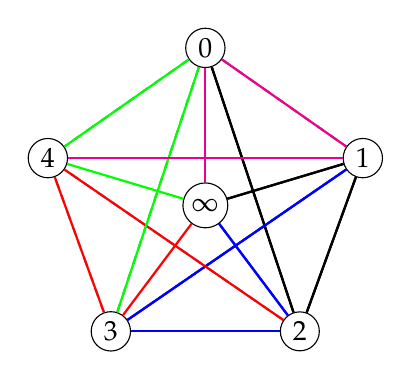
\begin{tikzpicture}[scale=0.2]
 \vertex(0) at (0,10) {0};
 \vertex(1) at (10,3) {1};
 \vertex(2) at (6,-8) {2};
 \vertex(3) at (-6,-8) {3};
 \vertex(4) at (-10,3) {4};
\vertex(5) at (0,0) {$\infty$};
\tikzset{EdgeStyle/.style={dashed,gray}} 
        \Edge(0)(1)
        \Edge(0)(2);
        \Edge(0)(3)
        \Edge(0)(4);
        \Edge(1)(2)
        \Edge(1)(3);
        \Edge(1)(4)
        \Edge(2)(3);
        \Edge(2)(4)
        \Edge(3)(4);
            \tikzset{EdgeStyle/.style={black}}
      \Edge(0)(2)
        \Edge(2)(1)
        \Edge(1)(5);
         \tikzset{EdgeStyle/.style={blue}}
      \Edge(1)(3)
        \Edge(2)(3)
        \Edge(2)(5);
         \tikzset{EdgeStyle/.style={black}}
      \Edge(0)(2)
        \Edge(2)(1)
        \Edge(1)(5); 
         \tikzset{EdgeStyle/.style={blue}}
      \Edge(1)(3)
        \Edge(2)(3)
        \Edge(2)(5);  
        \tikzset{EdgeStyle/.style={red}}
      \Edge(2)(4)
        \Edge(4)(3)
        \Edge(3)(5); 
        \tikzset{EdgeStyle/.style={green}}
      \Edge(3)(0)
        \Edge(4)(0)
        \Edge(4)(5);   
         \tikzset{EdgeStyle/.style={magenta}}
      \Edge(4)(1)
        \Edge(1)(0)
        \Edge(0)(5);
    \end{tikzpicture}
\end{center}
\end{column}%
\end{columns}
\end{frame}
%%------1-rot bipartite
\begin{frame}{Bipartite Graphs}
\begin{itemize}
    \item Recall the length of  $xy \in E(K_n)$ is min$(|x-y|,n-|x-y|).$
    \item A $\sigma$-labeling is a $\rho$-labeling such that the length of every edge $xy \in E(K_n)$ is $|x-y|.$
    \pause
    \item F and Tran introduced the following restricted $\sigma$-labeling in 2020.
\end{itemize}
\begin{definition}
 Let $G$ be a bipartite graph with $n$ edges and bipartition $V(G)=A\cup B$. A $\sigma^{+-}$-\emph{labeling} of $G$ is a $\sigma$-labeling with:
\begin{enumerate}
    \item $f(a)<f(b)$ for every edge $ab\in E(G)$ with $a\in A$ and $b \in B$
    \item $f(a)-f(b) \neq n$ for all $a,b \in V(G)$
    \item $f(v) \not \in \{2n-1,2n\}$ for all $v \in V(G)$
\end{enumerate}   
\end{definition}    

\end{frame}
%------------
\begin{frame}{Bipartite Graphs}
    \begin{theorem} [F, Tran, 2020] 
Let $G$ be a graph with $n$ edges and a $\sigma^{+-}$-labeling such that the edge of length $n$ is a pendant edge. Then there exists cyclic $G$-decompositions of $K_{2nt}$ and $K_{2nt+1}$ for every positive integer $t.$
\end{theorem}

\end{frame}

%-----------1-rot rho tripartite---------
\begin{frame}
\frametitle{Tripartite Graphs}
\begin{itemize}
\item Let $V(K_{2n})=\{0,1,2,...,2n-2,\infty\}.$\\
\pause
\item Let $G$ be a tripartite graph with $n$ edges, tripartition $\{A,B,C\}$, and pendant edge $xy$ with deg$(y)=1$.
\pause
\item
A \emph{1-rotational $\rho$-tripartite labeling} of $G$ is a 1-rotational $\rho$-labeling $f$ that:
\begin{enumerate}
    \item $f(y)=\infty.$
    \item $f(a)<f(v)$ for every edge $av$ with $a \in A.$
    \item For every edge $bc$ with $b \in B$ and $c \in C,$ there exists a complementary edge $b'c'$ with $b' \in B$ and $y' \in Y$ such that 
\[ |f(b)-f(c)|+|f(b')-f(c')|=2n.
\]
\end{enumerate}
\end{itemize}
\end{frame}
%%%---example
\begin{frame}
\frametitle{1-Rotational $\rho$-tripartite Labeling}
\begin{itemize}
\item Let $V(K_{2n})=\{0,1,2,...,2n-2,\infty\}$ and $G$ be a tripartite graph with $n$ edges, tripartition $\{A,B,C\}$, and pendant edge $xy$ with deg$(y)=1$.
\item
A \emph{1-rotational $\rho$-tripartite labeling} of $G$ is a 1-rotational $\rho$-labeling $f$ that:
\begin{enumerate}
    \item $f(y)=\infty.$
    \item $f(a)<f(v)$ for every edge $av$ with $a \in A.$
    \item For every edge $bc$ with $b \in B$ and $c \in C,$ there exists a complementary edge $b'c'$ with $b' \in B$ and $y' \in Y$ such that 
 $|f(b)-f(c)|+|f(b')-f(c')|=2n.$
\end{enumerate}
\end{itemize}
\begin{center}
    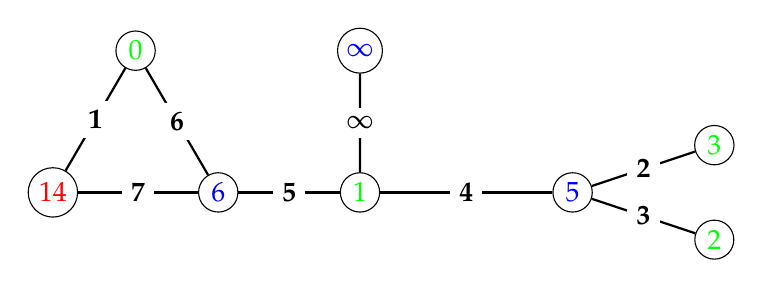
\begin{tikzpicture}[scale=0.3]
   \tikzstyle{vertex}=[circle, draw, inner sep=2pt, minimum size=10pt]
    
 \vertex(1) at (0,0) {\textcolor{red}{14}};
 \vertex(2) at (3.5,6) {\textcolor{green}{0}};
 \vertex(3) at (7,0) {\textcolor{blue}{6}};
 \vertex(4) at (13,0) {\textcolor{green}{1}};
 \vertex(5) at (13,6) {\textcolor{blue}{$\infty$}};
\vertex(6) at (22,0) {\textcolor{blue}{5}};
 \vertex(7) at (28,-2) {\textcolor{green}{2}};
 \vertex(8) at (28,2) {\textcolor{green}{3}};
\tikzset{EdgeStyle/.style={}} % insert --> in brackets for directed graph or bend right etc
        \Edge[label=\bf{1}](1)(2)
        \Edge[label=\bf{7}](1)(3)
        \Edge[label=\bf{6}](3)(2)
        \Edge[label=\bf{5}](4)(3)
        \Edge[label=\bf{$\infty$}](5)(4)
        \Edge[label=\bf{4}](4)(6)
        \Edge[label=\bf{3}](6)(7)
        \Edge[label=\bf{2}](6)(8);
    \end{tikzpicture}
\end{center}
\end{frame}

%-----1-rotational thm-----------
\begin{frame}{1-Rotational Designs}
 \begin{theorem}[Bunge, 2019]
 Let $G$ be a tripartite graph on $n$ edges with at least one pendant edge. If $G$ admits a 1-rotational $\rho$-tripartite labeling, then there exists a 1-rotational decomposition of $K_{2nt}$ for any positive integer $t.$
 \end{theorem}  
 \begin{center}
    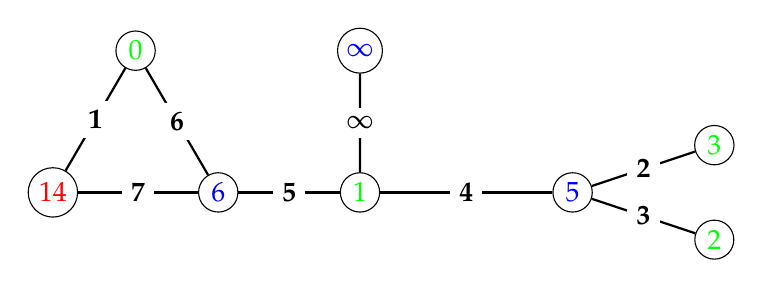
\begin{tikzpicture}[scale=0.3]
   \tikzstyle{vertex}=[circle, draw, inner sep=2pt, minimum size=10pt]
    
 \vertex(1) at (0,0) {\textcolor{red}{14}};
 \vertex(2) at (3.5,6) {\textcolor{green}{0}};
 \vertex(3) at (7,0) {\textcolor{blue}{6}};
 \vertex(4) at (13,0) {\textcolor{green}{1}};
 \vertex(5) at (13,6) {\textcolor{blue}{$\infty$}};
\vertex(6) at (22,0) {\textcolor{blue}{5}};
 \vertex(7) at (28,-2) {\textcolor{green}{2}};
 \vertex(8) at (28,2) {\textcolor{green}{3}};
\tikzset{EdgeStyle/.style={}} % insert --> in brackets for directed graph or bend right etc
        \Edge[label=\bf{1}](1)(2)
        \Edge[label=\bf{7}](1)(3)
        \Edge[label=\bf{6}](3)(2)
        \Edge[label=\bf{5}](4)(3)
        \Edge[label=\bf{$\infty$}](5)(4)
        \Edge[label=\bf{4}](4)(6)
        \Edge[label=\bf{3}](6)(7)
        \Edge[label=\bf{2}](6)(8);
    \end{tikzpicture}
\end{center}
\end{frame}
%----------6 edges
\section{Necessary Conditions and Tools}
\begin{frame}{Necessary Conditions}
\begin{observation}
    If $G$ is a graph with $6$ edges and a $G$-design of order $n$ exists, then $n \equiv 0,1,4, \; \text{or} \;9 \pmod{12}.$
\end{observation}
    \pause
    \begin{itemize}
        \item The Rosa-type labelings discussed so far will take care of $n \equiv 0 \; \text{or} \; 1 \pmod{12}$ only
        \begin{itemize}
            \item $\sigma^{+-}$ for the 27 bipartite graphs (23 forests and 4 unicyclics)
            \item $\rho$-tripartite and $1$-rotational $\rho$-tripartite for the 9 tripartite unicyclics
        \end{itemize}
        \pause
        \item What to do about $n \equiv 4 \; \text{or} \; 9 \pmod{12}$?
        \pause
        \item If the designs exist, they cannot be cyclic
        \begin{itemize}
            \item Ex. $K_{21}$ has $210=6 \times 35$ edges
        \end{itemize}
        \pause
        \item We'll adapt the techniques; click multiple blocks
    \end{itemize}
\end{frame}
%%%%%%%%%%%%%%%%%%%%%%%%%%%%%%%%%%%%%%%%%%%%%%
\section{Examples}
\begin{frame}{A Forest and $n=12k+4$}
    \centering
    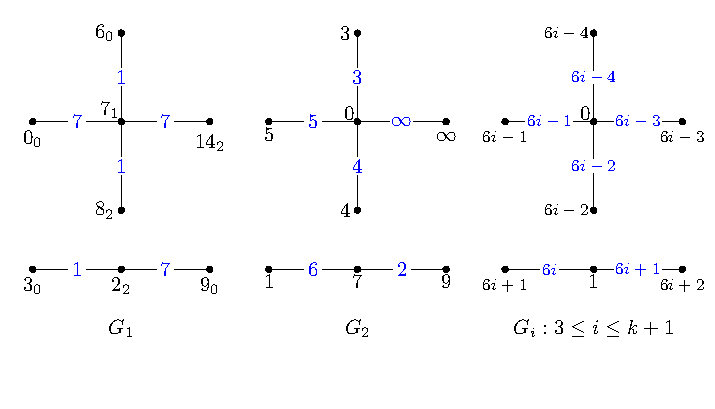
\includegraphics[scale=0.8]{Forest 4 mod 12.pdf}
    \pause 
    \begin{itemize}
        \item Click $G_1$ by $3$ and $G_i$ by $1$ for $2\leq i \leq k+1$ (we're working in $Z_{12k+3}$)
        \item Number of edges of each length $=3\times \frac{n-1}{3}=1\times (n-1)=n-1$
        \item Total number of edges $=(n-1)\times \frac{n}{2} =\binom{n}{2} $
    \end{itemize}
\end{frame}
%----------------
\begin{frame}{Approach for Tripartite Unicyclics and $n=12k+9$}
  \begin{itemize}
      \item Partition $V(K_n)$ into three \emph{groups} of cardinality $4k+3:$
      \[
\begin{array}{lll}
A&=&\{(0,0),(1,0),\dots,(4k+2,0)\}\\
B&=&\{(0,1),(1,1),\dots,(4k+2,1)\}\\
C&=&\{(0,2),(1,2),\dots,(4k+2,2)\}
\end{array}
\]
\item The edge set of $K_n$ can be expressed as
\[
  E(K_n) = \textcolor{red}{ \{(i,j)(i',j') : j=j', i\neq i'\}}    
    \cup \textcolor{blue}{\{(i,j)(i',j') : j\neq j'\}}
\]
\item \textcolor{red}{Intragroup edge} length defined as usual for $K_{4k+3}$
\item \textcolor{blue}{Intergroup edge} length defined as $\ell((i,j)(i',j+1))=i'-i$ where $i'-i$ is reduced modulo $4k+3$ and $j+1$ is taken modulo 3
\item Exactly one edge of each length can be obtained by clicking $3k+2$ blocks
  \end{itemize}
\end{frame}
%------------
\begin{frame}{Approach for Tripartite Unicyclics and $n=12k+4$}
  \begin{itemize}
      \item Partition $V(K_n)$ into $\{\infty\}$ and three \emph{groups} of cardinality $4k+1:$
      \[
\begin{array}{lll}
A&=&\{(0,0),(1,0),\dots,(4k,0)\}\\
B&=&\{(0,1),(1,1),\dots,(4k,1)\}\\
C&=&\{(0,2),(1,2),\dots,(4k,2)\}
\end{array}
\]
\item The edge set of $K_n$ can be expressed as before with the addition of $n-1$ edges of length $\infty.$
\item \textcolor{red}{Intragroup edges} take on lengths $\{1,2,\dots,2k\}$
\item \textcolor{blue}{Intergroup edges} take on lengths $\{0,1,\dots,4k\}$ between each pair of groups
  \end{itemize}
\end{frame}
%-----------
\begin{frame}{A $(C_3 \cup P_3 \cup P_2)$-design of order $12k+9$}
    \centering
    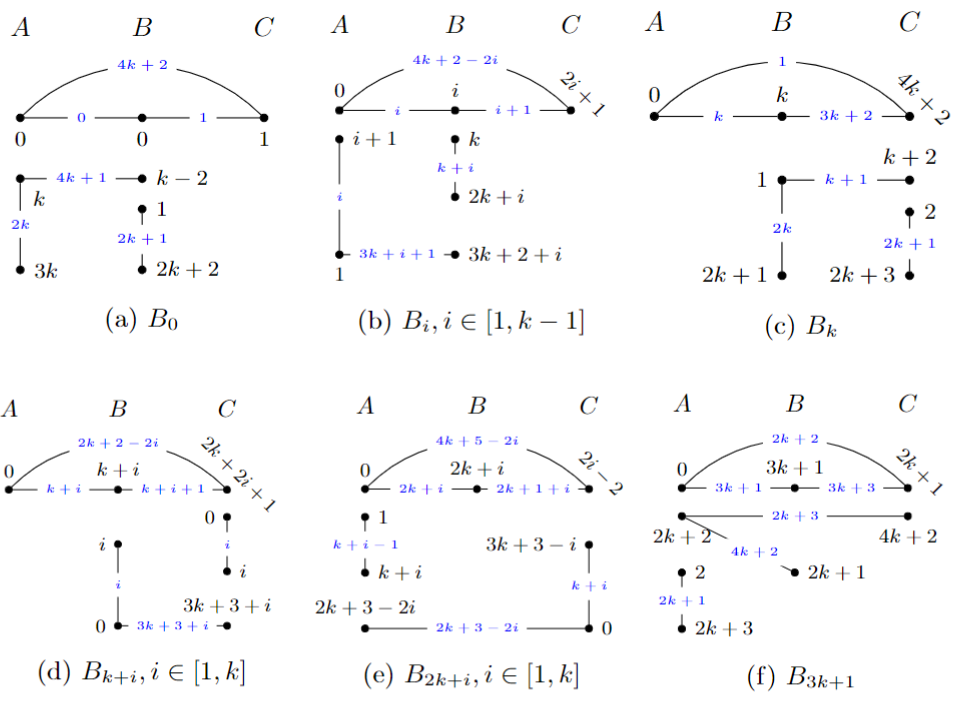
\includegraphics[scale=0.6]{9mod12 ex.PNG}
\end{frame}

%-------------------
\section{Main Result}
\begin{frame}{Main Result}
    \begin{theorem}[Ahern, F, Froncek, Keranen, Peters, 2022+]
        If $G$ is a disconnected graph with six edges, then a $G$-design of order $n$ exists if and only if $n \equiv 0,1,4, \; \text{or} \; 9 \pmod{12}$ unless either $n=4$ or $n=9$ and $G$ is isomorphic to one of the graphs listed below.
        \begin{itemize}
     \begin{multicols}{2}
        \item [$\square$] $K_{1,5} \cup K_2$
        \item [$\square$]$K_{1,4} \cup 2K_2$
        \item [$\square$]$K_{1,3} \cup 3K_2$
        \item [$\square$]$P_4 \cup 3K_2$
        \item [$\square$]$2P_3 \cup 2K_2$
        \item [$\square$]$P_3 \cup 4K_2$
        \item [$\square$]$6K_2$
        \item [$\square$]$K_3 \cup K_{1,3}$
        \end{multicols}
    \end{itemize}
    \end{theorem}
    \pause
   \textbf{THANK YOU!} 
\end{frame}

%------------------












%%The End
\end{document}
